\documentclass[oneside, 10pt]{article}

\usepackage{tcolorbox}
\usepackage{ulem} %math
\usepackage{amsmath}
\usepackage{amsfonts}
\usepackage{amssymb}
\usepackage{graphicx}
\usepackage{enumerate}


%Create a box for theorems
%\begin{theo}[titel] %optional
%tekst
%\end{theo}
\newenvironment{theo}[1][Vigtigt]{%
\begin{tcolorbox}[colback=green!5,colframe=green!40!black,title=\textbf{#1}]
}{%
\end{tcolorbox}
}




%Create a square matrix
%\begin{ArgMat}{2}
%21 & 22 & 23 \\  
%a & b & c
%\end{ArgMat}
%
% Info: http://tex.stackexchange.com/questions/2233/whats-the-best-way-make-an-augmented-coefficient-matrix
%
\newenvironment{ArgMat}{%
$
  \left[\begin{array}{@{}*{100}{r}r@{}}
}{%
  \end{array}\right]
  $
}

\newenvironment{deter}{%
$
  \left|\begin{array}{@{}*{100}{r}r@{}}
}{%
  \end{array}\right|
  $
}


%Create multiple lines with holes
%\begin{SysEqu}
%x_1 && &- &5x_3 &+ &2x_4=& 1 \\
%x_1 &+ &x_2 &+ &x_3 && =& 4 \\
%&&&&&&0 =& 0
%\end{SysEqu}
\newenvironment{SysEqu}{%
$  \setlength\arraycolsep{0.1em}
  \begin{array}{@{}*{100}{r}r@{}}
}{%
  \end{array}$
}

%Create solution for x_1, x_n...
%\begin{solu}
%x_1 &= d \\
%x_2 &= e \\
%x_3 &= s
%\end{solu}
\newenvironment{solu}{%
$
  \setlength\arraycolsep{0.1em}
  \left\{\begin{array}{@{}*{100}{r}r@{}}
}{%
  \end{array}\right.
$
}

\usepackage{lastpage}


\newcommand{\HRule}{\rule{\linewidth}{0.8mm}}

%Tekst i fotter
\newcommand{\footerText}{\thepage\xspace /\pageref{LastPage}}
\newcommand{\ProjectName}{433 MHz styring af AeroQuad}


\chapterstyle{hangnum}




\nouppercaseheads
\makepagestyle{mystyle} 

\makeevenhead{mystyle}{}{\\ \leftmark}{} 
\makeoddhead{mystyle}{}{\\ \leftmark}{} 
\makeevenfoot{mystyle}{}{\footerText}{} 
\makeoddfoot{mystyle}{}{\footerText}{} 
\makeatletter
\makepsmarks{mystyle}{% Overskriften på sidehovedet
  \createmark{chapter}{left}{shownumber}{\@chapapp\ }{.\ }} 
\makeatother
\makefootrule{mystyle}{\textwidth}{\normalrulethickness}{0.4pt}
\makeheadrule{mystyle}{\textwidth}{\normalrulethickness}

\makepagestyle{plain}
\makeevenhead{plain}{}{}{}
\makeoddhead{plain}{}{}{}
\makeevenfoot{plain}{}{\footerText}{}
\makeoddfoot{plain}{}{\footerText}{}
\makefootrule{plain}{\textwidth}{\normalrulethickness}{0.4pt}

\pagestyle{mystyle}

%%----------------------------------------------------------------------
%
%%Redefining chapter style
%%\renewcommand\chapterheadstart{\vspace*{\beforechapskip}}
%\renewcommand\chapterheadstart{\vspace*{10pt}}
%\renewcommand\printchaptername{\chapnamefont }%\@chapapp}
%\renewcommand\chapternamenum{\space}
%\renewcommand\printchapternum{\chapnumfont \thechapter}
%\renewcommand\afterchapternum{\space: }%\par\nobreak\vskip \midchapskip}
%\renewcommand\printchapternonum{}
%\renewcommand\printchaptertitle[1]{\chaptitlefont #1}
\setlength{\beforechapskip}{0pt} 
\setlength{\afterchapskip}{0pt} 
%\setlength{\voffset}{0pt} 
\setlength{\headsep}{25pt}
%\setlength{\topmargin}{35pt}
%%\setlength{\headheight}{102pt}
%\setlength{\textheight}{302pt}
\renewcommand\afterchaptertitle{\par\nobreak\vskip \afterchapskip}
%%----------------------------------------------------------------------




%Sidehoved og -fod pakke
%Margin
\usepackage[left=2cm,right=2cm,top=2.5cm,bottom=2cm]{geometry}
\usepackage{lastpage}



%%URL kommandoer og sidetal farve
%%Kaldes med \url{www...}
%\usepackage{color} %Skal også bruges
\usepackage{hyperref}
\hypersetup{ 
	colorlinks	= true, 	% false: boxed links; true: colored links
    urlcolor	= blue,		% color of external links
    linkcolor	= black, 	% color of page numbers
    citecolor	= blue,
}



%Mellemrum mellem linjerne    
\linespread{1.5}


%Seperated files
%--------------------------------------------------
%Opret filer således:
%\documentclass[Navn-på-hovedfil]{subfiles}
%\begin{document}
% Indmad
%\end{document}
%
% I hovedfil inkluderes således:
% \subfile{navn-på-subfil}
%--------------------------------------------------
\usepackage{subfiles}

%Prevent wierd placement of figures
%\usepackage[section]{placeins}

%Standard sti at søge efter billeder
%--------------------------------------------------
%\begin{figure}[hbtp]
%\centering
%\includegraphics[scale=1]{filnavn-for-png}
%\caption{Titel}
%\label{fig:referenceNavn}
%\end{figure}
%--------------------------------------------------
\usepackage{graphicx}
\usepackage{subcaption}
\usepackage{float}
\graphicspath{{../Figures/}}

%Speciel skrift for enkelt linje kode
%--------------------------------------------------
%Udskriver med fonten 'Courier'
%Mere info her: http://tex.stackexchange.com/questions/25249/how-do-i-use-a-particular-font-for-a-small-section-of-text-in-my-document
%Eksempel: Funktionen \code{void Hello()} giver et output
%--------------------------------------------------
\newcommand{\code}[1]{{\fontfamily{pcr}\selectfont #1}}


% Følgende er til koder.
%----------------------------------------------------------
%\begin{lstlisting}[caption=Overskrift på boks, style=Code-C++, label=lst:referenceLabel]
%public void hello(){}
%\end{lstlisting}
%----------------------------------------------------------

%Exstra space
\usepackage{xspace}
%Navn på bokse efterfulgt af \xspace (hvis det skal være mellemrum
%gives det med denne udvidelse. Ellers ingen mellemrum.
\newcommand{\codeTitle}{Kodeudsnit\xspace}

%Pakker der skal bruges til lstlisting
\usepackage{listings}
\usepackage{color}
\usepackage{textcomp}
\definecolor{listinggray}{gray}{0.9}
\definecolor{lbcolor}{rgb}{0.9,0.9,0.9}
\renewcommand{\lstlistingname}{\codeTitle}
\lstdefinestyle{Code}
{
	keywordstyle	= \bfseries\ttfamily\color[rgb]{0,0,1},
	identifierstyle	= \ttfamily,
	commentstyle	= \color[rgb]{0.133,0.545,0.133},
	stringstyle		= \ttfamily\color[rgb]{0.627,0.126,0.941},
	showstringspaces= false,
	basicstyle		= \small,
	numberstyle		= \footnotesize,
%	numbers			= left, % Tal? Udkommenter hvis ikke
	stepnumber		= 2,
	numbersep		= 6pt,
	tabsize			= 2,
	breaklines		= true,
	prebreak 		= \raisebox{0ex}[0ex][0ex]{\ensuremath{\hookleftarrow}},
	breakatwhitespace= false,
%	aboveskip		= {1.5\baselineskip},
  	columns			= fixed,
  	upquote			= true,
  	extendedchars	= true,
 	backgroundcolor = \color{lbcolor},
	lineskip		= 1pt,
%	xleftmargin		= 17pt,
%	framexleftmargin= 17pt,
	framexrightmargin	= 0pt, %6pt
%	framexbottommargin	= 4pt,
}

%Bredde der bruges til indryk
%Den skal være 6 pt mindre
\usepackage{calc}
\newlength{\mywidth}
\setlength{\mywidth}{\textwidth-6pt}


% Forskellige styles for forskellige kodetyper
\usepackage{caption}
\DeclareCaptionFont{white}{\color{white}}
\DeclareCaptionFormat{listing}%
{\colorbox[cmyk]{0.43, 0.35, 0.35,0.35}{\parbox{\mywidth}{\hspace{5pt}#1#2#3}}}
\captionsetup[lstlisting]
{
	format			= listing,
	labelfont		= white,
	textfont		= white, 
	singlelinecheck	= false, 
	width			= \mywidth,
	margin			= 0pt, 
	font			= {bf,footnotesize}
}

\lstdefinestyle{Code-C} {language=C, style=Code}
\lstdefinestyle{Code-Java} {language=Java, style=Code}
\lstdefinestyle{Code-C++} {language=[Visual]C++, style=Code}
\lstdefinestyle{Code-VHDL} {language=VHDL, style=Code}
\lstdefinestyle{Code-Bash} {language=Bash, style=Code}

%Text typesetting
%--------------------------------------------------------
%\usepackage{baskervald}
\usepackage{lmodern}
\usepackage[T1]{fontenc}              
\usepackage[utf8]{inputenc}         
\usepackage[english]{babel}       

\setlength{\parindent}{0pt}
\nonzeroparskip

%\setaftersubsecskip{1sp}
%\setaftersubsubsecskip{1sp}
 


%Dybde på indholdsfortegnelse
%----------------------------------------------------------
%Chapter, section, subsection, subsubsection
%----------------------------------------------------------
\setcounter{secnumdepth}{3}
\setcounter{tocdepth}{3}


%Tables
%----------------------------------------------------------
\usepackage{tabularx}
\usepackage{array}
\usepackage{multirow} 
\usepackage{multicol} 
\usepackage{booktabs}
\usepackage{wrapfig}
\renewcommand{\arraystretch}{1.5}



%Misc
%----------------------------------------------------------
\usepackage{cite}
\usepackage{appendix}
\usepackage{amssymb}
\usepackage{url,ragged2e}
\usepackage{enumerate}
\usepackage{amsmath} %Math bibliotek


\usepackage{longtable}


\title{Middleware and Communication -- exercises}
\author{Rasmus Bækgaard}
\date{}

\begin{document}
\maketitle


\section{Exercise 1}
\subsection{Determinism and real-time}
\begin{enumerate}
	\item Discuss how deterministic finite automata (DFA) define determinism
	\item[] 
	
	\item Discuss how non-deterministic finite automata (NFA) define non-determinism
	\item[]

	\item I modsætning til DFA og NFA bruger TFA tiden som faktor.
	Derudover har TFA ikke et $Q$ med finite state, men $L$ med finite sets of locations (minder dog om). 
	$L_0$ er i $L$ som start placering og $L_F$ som slutplacering.
	$C$ er et finite set af clocks og $E$ udregnes med hensyn til de clocks der måtte være i systemet.
	TFA har en local clock invariant (de små bobler med hensyn til forskellige clocks).

	\item Det er tilladt. Dette skyldes, at $E \in \ldots ( \Sigma \cup \{ \epsilon \}) \ldots$. En empty string kan resultere i, at systemet skifter state uden input (se L1S14) -- non-deterministic.

	\item  Discuss why TFA can be used to model distributed real-time systems.
	\item[] Man kan kun komme i et state, fordi man har sine clock constraints, $\Phi(C)$

	\item  Discuss the relationship between (non)determinism and dead-line guarantees in real-time systems.
	\item[] I et deterministisk system er der kun den ene vej, som vil ende i dit mål, men ikke garanteret inden for dead-line. 
	I et non-deterministisk system kan du splitte dig op i flere veje og ikke nødvendigvis nå de mål overhovedet (og ikke inden for tiden), men det er muligt at garantere.
\end{enumerate}

Precision Time Protocol
\begin{enumerate}
	\item Discuss whether the Precision Time Protocol (PTP) is deterministic
	\item[] Ja -- Selve protokollen er, men fordi man kan have asynmetrisk delay (delay frem og tilbage er det samme) og ikke-trådet netværk.

	\item Discuss what a packet-switched network is
	\item[]  Data i små pakker, der har en adresse på sig. 
	På denne måde kan flere bruge samme linje og kun se det, der er relevant for en selv.

	\item  Discuss to what extent the PTP is tailored for packet-switched networks only
	\item[] Master sender 2 pakker, som alle kan modtage. 
	PTP synkroniserer på Slave-side og mange slaves kan modtage de 2 pakker (kaldet "multi cast").

	\item Discuss whether the PTP works on Ethernet only
	\item[] It works on all packet-switched networks.

	\item Discuss how the PTP can support real-time operations on Ethernet
	\item[] Kun operationer, som siger "gør noget klokken $X$" er realtid.
	Pakker ankommer ikke i realtid. 

	\item Discuss the offset correction and delay correction in the PTP
	\item[] Offset: Forskellen mellem Master-tid og Slave-tid.
	\item[] Delay: Korrektion med Slave request og respond

	\item Discuss whether it is fair to assume a symmetric line delay in the delay correction
	\item[]

	\item Discuss how the PTP can play a role in Long Term Evolution (LTE) and LTE Advanced
	\item Sketch and discuss a DFA, NFA or TFA that models the PTP
\end{enumerate}

\section{Article}
\begin{itemize}
	\item Har forfatterne lavet andre, citerede artikler?
	\item SyncE -- clock går lige igennem PHY-laget.
	\item Se slides
\end{itemize}










\section{Exercises 2}

\subsection{Single segment Ethernet}

\begin{enumerate}
	\item  Discuss the cause of non-determinism in single segment Ethernet
	\item [] Implementationsmetoden svarer til en hub -- et single shared medium, og collission kunne resultere i store forsinkelser (Deraf non-deterministisk).

	\item  Discuss the functioning of CSMA/CD and in particular the Back-Off Algorithm (BOA)
	\item [] Carrier Send Multiple Access / Collision detection
	\item [] Giver collissions, hvilket resulterer i Back-Off algoritmen, hvor en forbindelse får et lille delay og prøver igen (og rekursiv med større delay). 
	Hvis ikke der er sendt noget efter $x$ antal gange vil den stoppe helt med at sende.

	\item  Discuss medium monopolization – and the likelihood thereof – by BOA
	\item [] Dette er worst-case scenariet for Back-Off algoritmen, hvor én node bliver ved med at sende og andre noder må vige.

	\item  State the expected back-off time in BOA as a function of collisions, i.e. E(c)
	\item [] $E(c) = r \cdot t_{slot},$ where $r \sim \mathcal{U}[0, \ldots, 2^c-1], t_{slot} = 51.2 \mu s $ at $10 \frac{Mbit}{s} $ eller $ 5.12 \mu s$ at $100 \frac{Mbit}{s}, c \leq 10 $ (L2S21).
	\item [] $E(c) = \bigg(\sum\limits_{i=0}^c \frac{1}{c+1} \cdot (2^c-1)\bigg) \cdot t_{slot}$

	\item  What is the maximum back-off time when the truncation occurs after c = 10 collisions?
	\item[] $E(10) = (2^{10} - 1) \cdot t_{slot}$

	\item  Sketch a NFA that models non-determinism in single segment Ethernet
	\item[] See Figure \ref{fig:NFA}.

\end{enumerate}
\begin{figure}[hbtp]
\centering
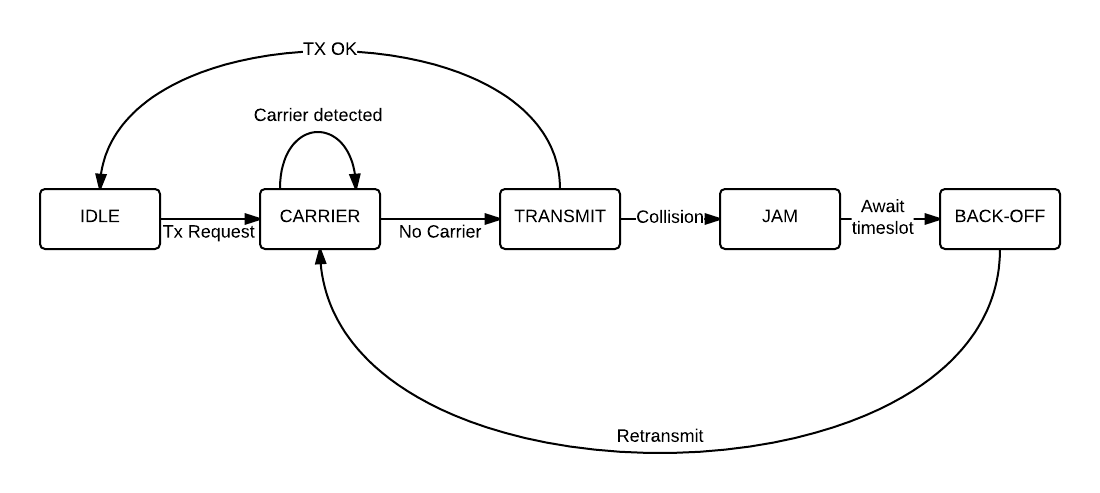
\includegraphics[width=0.9 \textwidth]{NFA}
\caption{NFA for non-determinism in single segment Ethernet}
\label{fig:NFA}
\end{figure}



\subsection{Switched Ethernet}
\begin{enumerate}
	\item 1. Discuss the benefits of micro-segmentation
	\item[]
	
	\item 2. What kind of network device offer micro-segmentation capabilities?
	\item[]
	
	\item 3. Discuss the role of CSMA/CD in fully switched (full duplex) Ethernet
	\item[]
	
	\item 4. Why are latency and packet delay variations of concern in switched Ethernet?
	\item[]

	\item 5. How may latency and packet delay variations influence dead-line guarantees of a real-time system based on Ethernet?
	\item[]
	
	\item 6. How does overflow and overflow prevention in switches impact predictability of worst-case transmission time bounds?
	\item[]
	
	\item 7. Discuss the purpose of the Spanning Tree algorithm
	\item[]
	
\end{enumerate}

\subsection{Real time Ethernet}

\begin{enumerate}
	\item 1. Discuss the motivation for having Ethernet as a field-bus technology
	\item[]
	
	\item 2. Discuss the relevance of leaving bandwidth for normal asynchronous traffic in real-time Ethernet deployments
	\item[]
	
	\item 3. Discuss the Ethernet Frame structure and how it supports real-time Ethernet methods
	\item[]
	
	\item 4. Discuss the real-time facilitating techniques applied in ProfinetIRT, EtherCAT, Ethernet Powerlink, Sercos III, and EtherNet/IP
	\item[]
	
	\item 5. How is overhead/payload ratio reduced in EtherCat?
	\item[]
	
	\item 6. Why is the Precision Time Protocol important to Ethernet/IP?
	\item[]
	
	\item 7. Discuss the Leaky Bucket algorithm and how it is relevant to real-time Ethernet
	\item[]
	
\end{enumerate}
	




\end{document}